\documentclass[a4paper,12pt]{article}                                         			% Font size, layout, paper format, document type
\usepackage[left=2.54cm,right=2.54cm,top=2.54cm,bottom=2.54cm,includehead]{geometry}    % Page margin settings
\usepackage[english]{babel}                                                   			% English hyphenation
\usepackage[utf8]{inputenc}                                                   			
\usepackage[hyperfootnotes=false]{hyperref}                                   			% PDF output [do not link footnotes]
\usepackage[nottoc]{tocbibind}                                                			% Table of contents extension (hide TOC itself)
\usepackage{makeidx}                                                          			% Index
\usepackage[intoc]{nomencl}                                                   			% Abbreviations index
\usepackage{fancyhdr}  																	% Fancy Header
\usepackage{csquotes}
\usepackage[style=apa, backend=biber]{biblatex}
\DeclareLanguageMapping{english}{english-apa}
\addbibresource{literatur/References.bib}
\usepackage{amsmath}                                                          			% Reset table and figure numbering per section
\usepackage[labelfont=bf,aboveskip=1mm]{caption}                              			% Figure and table captions (bold)
\usepackage{setspace}                                                         			% Line spacing (load before footmisc!)
\usepackage[bottom,multiple,hang,marginal]{footmisc}                          			% Footnotes [align at bottom, separate by separator for multiple footnotes]
\usepackage{graphicx}  % Graphics
\usepackage{pdfpages}
\usepackage{tabularx}                                                         			% Extended tables
\usepackage{longtable}                                                        			% Multi-page tables
\usepackage{color}                                                            			% Colors
\usepackage{enumitem}                                                         			% Command setlist (set line spacing for itemize environment to 1)
\usepackage{listings}                                                         			% Source code
\usepackage{zref}                                                        				% References (appendix references)
\usepackage[toc,style=altlist,translate=false]{glossaries}                    			% Glossary (after hyperref, inputenc, babel)
\usepackage{glossaries-babel}                                                 			% Glossary: translation in TOC
\usepackage{svg}
\usepackage{float}
\usepackage{appendix}

%%%%%%%%%%%%%%%%%%%%%%%% Define custom colors %%%%%%%%%%%%%%%%%%%%%%%%%%%%%%%
\definecolor{boxgray}{gray}{0.9}         % Background color for quote boxes
\definecolor{commentgray}{gray}{0.5}     % Gray for comments in source code
\definecolor{darkgreen}{rgb}{0,.5,0}     % Green for strings in source code

%%%%%%%%%%%%%%%%%%%%%%%% Define custom commands %%%%%%%%%%%%%%%%%%%%%%%%%%%%%
% Definition of \gqq{#1: text}: Text in quotation marks
\newcommand{\gqq}[1]{\glqq #1\grqq}

% Definition of \footref{#1: label}
% Reference to already existing footnotes using
\providecommand*{\footref}[1]{
	\begingroup
		\unrestored@protected@xdef\@thefnmark{\ref{#1}}
	\endgroup
\@footnotemark}

% Definition of \mypageref{#1: label}
% Combination of \ref{#1: label} and \pageref{#1: label}
\newcommand{\mypageref}[1]{\ref{#1} on page \pageref{#1}}

% Definition of \myboxquote{#1: text}
% Gray-shaded quotation environment (for quotes)
\newcommand{\myboxquote}[1]{
	\begin{quotation}
		\colorbox{boxgray}{\parbox{0.78\textwidth}{#1}}
	\end{quotation}
	\vspace*{1mm}
}

\makeatletter
\zref@newprop*{appsec}{}
\zref@addprop{main}{appsec}

% Definition of \applabel{#1: label}{#2: text}
% Used by \appsec{#1: text}{#2: label} to generate the label
\def\applabel#1#2{%
	\zref@setcurrent{appsec}{#2}%   
	\zref@wrapper@immediate{\zref@label{#1}}%
}

% Definition of \appref{#1: label}
% Use instead of \ref{#1: label} to refer to appendices
\def\appref#1{%
	\hyperref[#1]{\zref@extract{#1}{appsec}}%
}
\makeatother

% Definition of \appsection{#1: text}{#2: label}
% Replaces \section{#1: text} and \label{#2: label} for appendices
\newcommand{\theappsection}[1]{Appendix \Alph{section}:~\protect #1}
\newcommand{\appsection}[2]{
	\addtocounter{section}{1}
	\phantomsection
	\addcontentsline{toc}{section}{\theappsection{#1}}
	\markboth{\theappsection{#1}}{}

	\section*{\theappsection{#1}}
	\applabel{#2}{Appendix \Alph{section}}
	\label{#2}
}

%%%%%%%%%%%%% Generate index, abbreviations list, and glossary %%%%%%%%%%%%%%
\makeindex
\makenomenclature
\makeglossaries

% Specify citation style (Harvard method: Author + Year abbreviation) %
%\bibliographystyle{plainnat}

%%%%%%%%%%%%%%%%%%%%%%%%%%%%%%% PDF Optionsup{
	bookmarksopen=false,
	bookmarksnumbered=true,
	bookmarksopenlevel=0,
	pdftitle=\myTopic,
	pdfsubject=\myTopic,
	pdfauthor=\myAutor,
	pdfborder=0,
	pdfstartview=Fit,
	pdfpagelayout=SinglePage
}

% Header and footer
\pagestyle{fancy}
\fancyhf{}
\fancyhead[R]{\thepage}                         % Header right or outer
\renewcommand{\headrulewidth}{0.5pt}            % Header right or outer

% Layout and captions
\onehalfspacing                % Line spacing: 1.5 (default: 1.2)
\setlist{noitemsep}            % Set line spacing for items to 1

\addto\captionsngerman{        % Change table and figure captions
  \renewcommand{\figurename}{Fig.}
  \renewcommand{\tablename}{Tab.}
}
\numberwithin{table}{section}                               % Reset table numbering per section
\numberwithin{figure}{section}                              % Reset figure numbering per section
\renewcommand{\thetable}{\arabic{section}.\arabic{table}}   % Table numbering with section
\renewcommand{\thefigure}{\arabic{section}.\arabic{figure}} % Figure numbering with section
\renewcommand{\thefootnote}{\arabic{footnote}}              % Remove section label from footnotes

\renewcommand{\multfootsep}{, }                             % Separate multiple footnotes with ", "

% Listing style
\lstset{
	basicstyle=\ttfamily\scriptsize,
	commentstyle=\color{commentgray}\textit,
	showstringspaces=false,
	stringstyle=\color{darkgreen},
	keywordstyle=\color{blue},
	numbers=left,
	numberstyle=\tiny,
	stepnumber=1,
	numbersep=15pt,
	tabsize=2,
	fontadjust=true,
	frame=single,
	backgroundcolor=\color{boxgray},
	captionpos=b,
	linewidth=\linewidth,
	xleftmargin=0pto,
	breaklines=true,
	aboveskip=16pt
}
    

% Cover
\begin{document}
	\pagenumbering{Roman}
    \begin{titlepage}
    \centering
    \vspace*{2cm}
    {\Huge \textbf{A Review of the Literature}}\\
    \vspace{0.5cm}
    {\Huge\textbf{on Generative Agents:}}\\
    \vspace{1cm}
    {\Large Capabilities and Limitations}\\
    
    \vspace{4cm}
    
\includegraphics[width=0.3\textwidth]{dhwb_logo.png}
    \vspace{2cm}
    
    {Francisco Rodriguez Müller, on \today}
    \vspace{2cm}\\
    {Matriculation Number: 2775857, Course: {RV-WWIBE122}}\\
    {\small Supervisor: {Prof. Dr. Michael Bächle} \\ Modul: {Integrationsseminar}}\\

    \vfill
    {Wirtschaftsinformatik - Business Engineering}\\
    {Duale Hochschule Baden-Württemberg}\\
    {Ravensburg}
    \end{titlepage}
	\pagestyle{fancy}
	%\begin{titlepage}
	\begin{center}
		\vspace*{1cm}
		\Huge\bf Non-Disclosure Clause\\
		\vspace*{2cm}
		\normalsize\rm
		\begin{quotation}
			\parbox{0.8\textwidth}{The present \ifcase\myType seminar paper \or project report \or bachelor thesis\else\fi ~contains internal confidential information of the company \myCompany, \myCompanyAddressStreet, \myCompanyAddressCity. The dissemination of the content of the work in whole or in part is strictly prohibited. No copies or transcripts - including digital forms - may be made. Exceptions require the written approval of the company \myCompany, \myCompanyAddressStreet, \myCompanyAddressCity.}
		\end{quotation}
		\vspace*{1cm}
		\begin{quotation}
		  \parbox{0.8\textwidth}{
		  \begin{tabularx}{0.78\textwidth}{l@{\extracolsep\fill}l}
				\rule{4cm}{0.3mm}&\rule{4cm}{0.3mm}\\
	    	Place, Date&Signature
			\end{tabularx}}
		\end{quotation}
	\end{center}
\end{titlepage}
\newpage
\setcounter{page}{3}

	\include{pages/12_inhaltsverzeichnis}
	%\renewcommand{\nomname}{List of Abbreviations}
\setlength{\nomlabelwidth}{.25\hsize}
\renewcommand{\nomlabel}[1]{#1 \dotfill}
\setlength{\nomitemsep}{-\parsep}
\printnomenclature
\newpage

	%\include{pages/14_glossar}
	%S\include{pages/15_abbildungsverzeichnis}
	%\include{pages/16_tabellenverzeichnis}
	%\include{pages/17_listingsverzeichnis}

	% Chapters
	\pagestyle{fancy}
	\fancyhead[L]{\nouppercase{\rightmark}}                               % Header left or inner
	\pagenumbering{arabic}
	\include{Chapter/01_Introduction}
	%\include{Chapter/02_Theory}
	%\include{Chapter/03_Method}
	%\include{Chapter/04_Implementation}
	%\include{Chapter/05_Conclusion}
	
	
    %\include{Chapter/07anhang}
		
	% Appendix
	\renewcommand{\thetable}{\Alph{section}.\arabic{table}}              % Table numbering with section
	\renewcommand{\thefigure}{\Alph{section}.\arabic{figure}}            % Figure numbering with section
	\renewcommand{\thelstlisting}{\Alph{section}.\arabic{lstlisting}}    % Listing numbering with section
	% Completion
	%\bibliography{literatur/References}
\printbibliography[heading=bibintoc, title={References}]
\newpage
	\include{pages/19_index}
	\thispagestyle{empty}
\addcontentsline{toc}{section}{Declaration of Authenticity}
\begin{center}
	\vspace*{2cm}
	\Huge\bf Declaration of Authenticity\\
	\vspace*{3cm}
	\normalsize\rm
	I hereby declare that I have independently written my \ifcase\myType seminar paper \or project report \or bachelor's thesis\else\fi ~with the topic\\
	\vspace*{2cm}
	\Large\textbf{A Review of the Literature on Generative Agents}: Capabilities and Limitations \\
	\vspace*{2cm}
	\normalsize\rm
	and that I have not used any sources or aids other than those indicated.\\
	\vfill
	\begin{tabularx}{\textwidth}{l@{\extracolsep\fill}r}
  	\rule{7cm}{0.3mm}&\rule{7.55cm}{0.3mm}\\
	\end{tabularx}
	\begin{tabularx}{\textwidth}{*{2}{>{\arraybackslash}X}}
	  Place, Date&Signature\\
	\end{tabularx}
\end{center}
        \begin{appendix}
        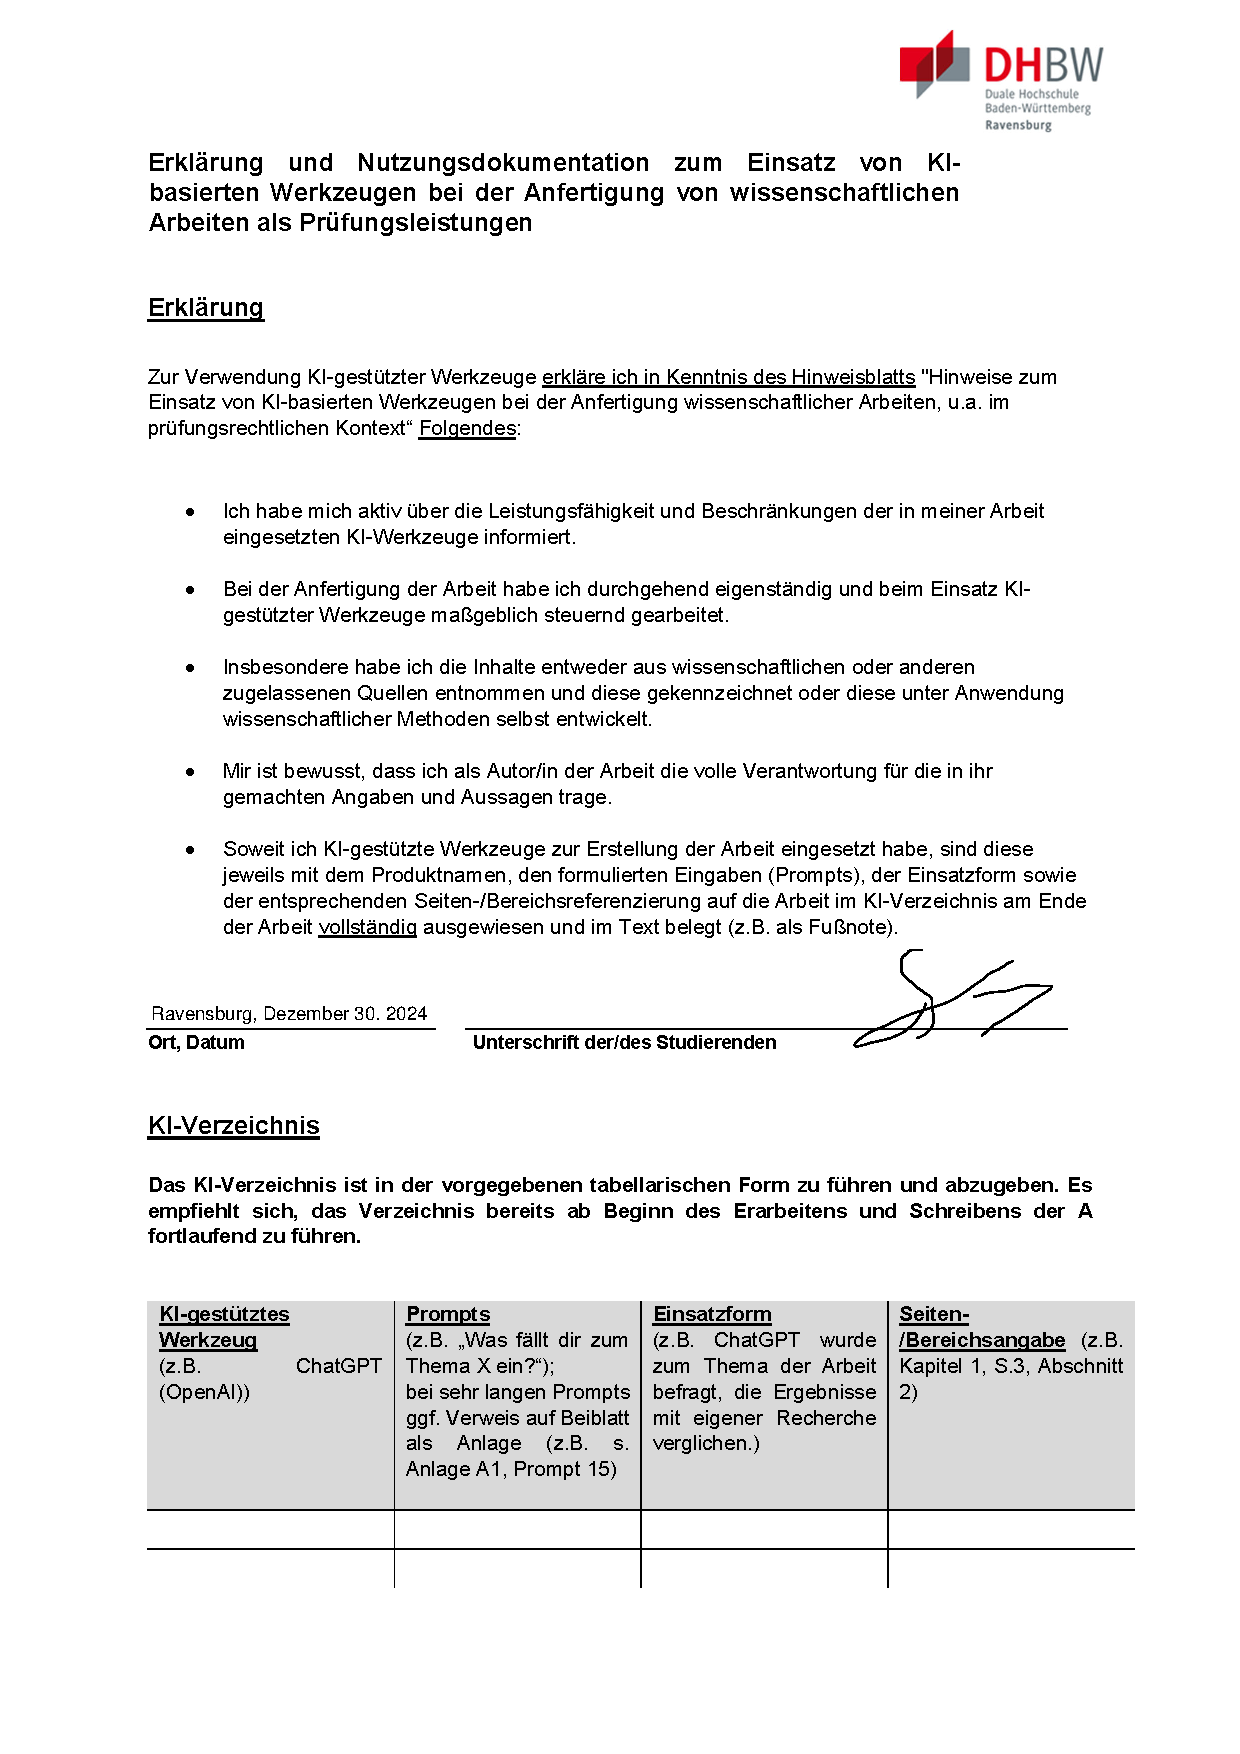
\includepdf{pages/24_02_21_Formular Hilfsmittelangabe KI_Wirtschaft.pdf}
	\end{appendix}
\end{document}

%%%%%%%%%%%%%%%%%%%%%%%%%%%%%%%%%%%%%%%%%%%%%%%%%%%%%%%%%%%%%%%%%%%%%%%%%%%%%
%%                                                                         %%
%% /\   /\         Do not make changes above this point            /\   /\ %%
%%                                                                         %%
%%%%%%%%%%%%%%%%%%%%%%%%%%%%%%%%%%%%%%%%%%%%%%%%%%%%%%%%%%%%%%%%%%%%%%%%%%%%%